\chapter{Methods} % Main chapter title

\label{Chapter:Methods}

The study is based on a systematic review of secondary data. The term secondary data is used in this study to refer to data that are used to address research questions that are different from the ones the original collector sought to answer (Vartanian, 2011). The search for the secondary data was guided by phrases such as: a) urban agricultural practices, b) indicators for the measurement of sustainable cities, c) economic, social and environmental benefits of urban agriculture, and d) negative effects of urban agriculture on the city. At the end of the search, 189 articles/reports/books related to urban agriculture and sustainable cities were used.

The literature on indicators for sustainable cities was screened for commonalities and differences towards building a conceptual framework, which was used to analyse the nexus between urban agriculture and sustainable cities. The conceptual framework was developed from the following models: a) the Green City Index (Supplementary Table 1), b) the Global City Indicators Facility (Supplementary Table 2) and c) Global Compact Cities Circles of Sustainability (Supplementary Table 3). The framework integrates the strengths of each model and together addresses the inherent weaknesses of a single model. The indicators were then categorised into three, namely economic, social and environmental to reflect the concept of sustainable development (Fig. \ref{fig:sustainableCityFramework}). The three dimensions are referred to as themes in this article. The literature was analysed by subjecting each of the content analysed to the specific indicators under the sustainable city themes.

\begin{figure}[th]
\centering

\includegraphics[width=1.00\textwidth]{./Figures/sustainableCityFramework.png}
\decoRule
\caption[Sustainable City Framework]{Sustainable City Framework.}
\label{fig:sustainableCityFramework}
\end{figure}

The literature was drawn from several geographical locations with different agro-climatic, economic, social and environmental characteristics. Lessons from these places underscore the importance of urban agriculture to the sustainable city discourse. For instance, in the global north, the importance of urban agriculture is more environmental in nature than socio-economic. However, the social and economic functions of urban agriculture are more pronounced in the cities in the global south. Despite these differences, the conceptual framework in the present study brings together economic, social and ecological indicators and can be applied in every city. The selection of the crops to cultivate to achieve the sustainability goals would however be based on the local climatic conditions.

%\begin{figure}[th]
%\centering
%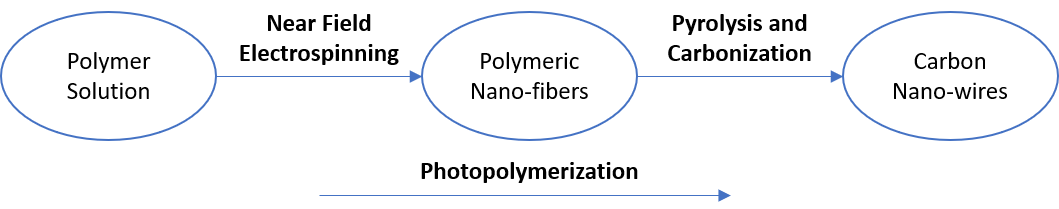
\includegraphics[width=0.95\textwidth]{./Figures/FabricationProcess.png}
%\decoRule
%\caption[Carbon Nano-wires Fabrication Process]{Fabrication process of carbon nano-wires to achieve through the proposed dissertation.}
%\label{fig:fabricationFlowChart}
%\end{figure}

%\begin{equation}
%\left(\tau _t^e-\frac{\tau _n^e \text{dr}}{\text{dz}}\right) 2 \pi  r+\frac{d \left(\pi  r^2
%   \left(\tau _{\text{zz}}-p\right)\right)}{\text{dz}}+\frac{\gamma  \text{dr} 2 \pi  r}{r
%   \text{dz}}+\rho  g \pi  r^2=\frac{d \left(\rho  \pi  r^2 v^2\right)}{\text{dz}}
%\label{eq:linearMomentum}
%\end{equation}